\documentclass[a4paper]{article}
\usepackage{graphicx} % Required for inserting images
\usepackage[utf8]{inputenc}
\usepackage{amsthm}
\usepackage{amsmath}
\usepackage{csquotes}
\usepackage{times} % Required for setting the font to Times New Roman
\usepackage{setspace} % Required for setting custom line spacing
\usepackage{url}
\usepackage{float}
\usepackage{amssymb}
\usepackage{amsmath} % enables text input in equations
\usepackage{float, eurosym, amssymb, color}
\usepackage{booktabs, cellspace}
\usepackage{adjustbox}
\usepackage{environ}
\usepackage{tikz}
\usepackage{geometry}
\usepackage{parskip}
\usepackage{MnSymbol}
\usepackage{parskip}
\usepackage[
    backend=biber, 
    natbib=true,
    style=numeric,
    sorting=none
]{biblatex} 
\usepackage{hyperref} 

%%%%%%%%%%%%% Page layout
\topmargin-20mm
\headheight10mm
\headsep10mm
\topskip0.1mm
\hoffset-15mm
\textwidth15.5cm
\textheight22cm
\parindent0em
%\markleft{\authors}
%\markright{\shorttitle} 
\pagenumbering{arabic}
%%%%%%%%%%%%%%%%%%

\addbibresource{references.bib}

\newcommand{\mX}{\mathcal{X}}

\usetikzlibrary{calc,cipher,sponge}
\makeatletter
\newsavebox{\measure@tikzpicture}
\NewEnviron{scaletikzpicturetowidth}[1]{%
  \def\tikz@width{#1}%
  \def\tikzscale{1}\begin{lrbox}{\measure@tikzpicture}%
  \BODY
  \end{lrbox}%
  \pgfmathparse{#1/\wd\measure@tikzpicture}%
  \edef\tikzscale{\pgfmathresult}%
  \BODY
}
\makeatother
\setstretch{1.25}


\date{May 2024}

\title{Lightweight Cryptography: Challenges and Approaches}
\author{
  Aitaza, A. \\
  \texttt{aka2973@thi.de}
  \and
  Öztürk O.\\
  \texttt{ozo8678@thi.de}   
  \and
  Topouzakis, A. \\
  \texttt{ant8751@thi.de}
  \and
  Maugueret, A. D.\\
  \texttt{adm5462@thi.de}
  }
  
\begin{document}
\maketitle

\newpage
\tableofcontents
\listoffigures
\newpage

\section{Notation}

\begin{figure}[H] 
    \centering 
    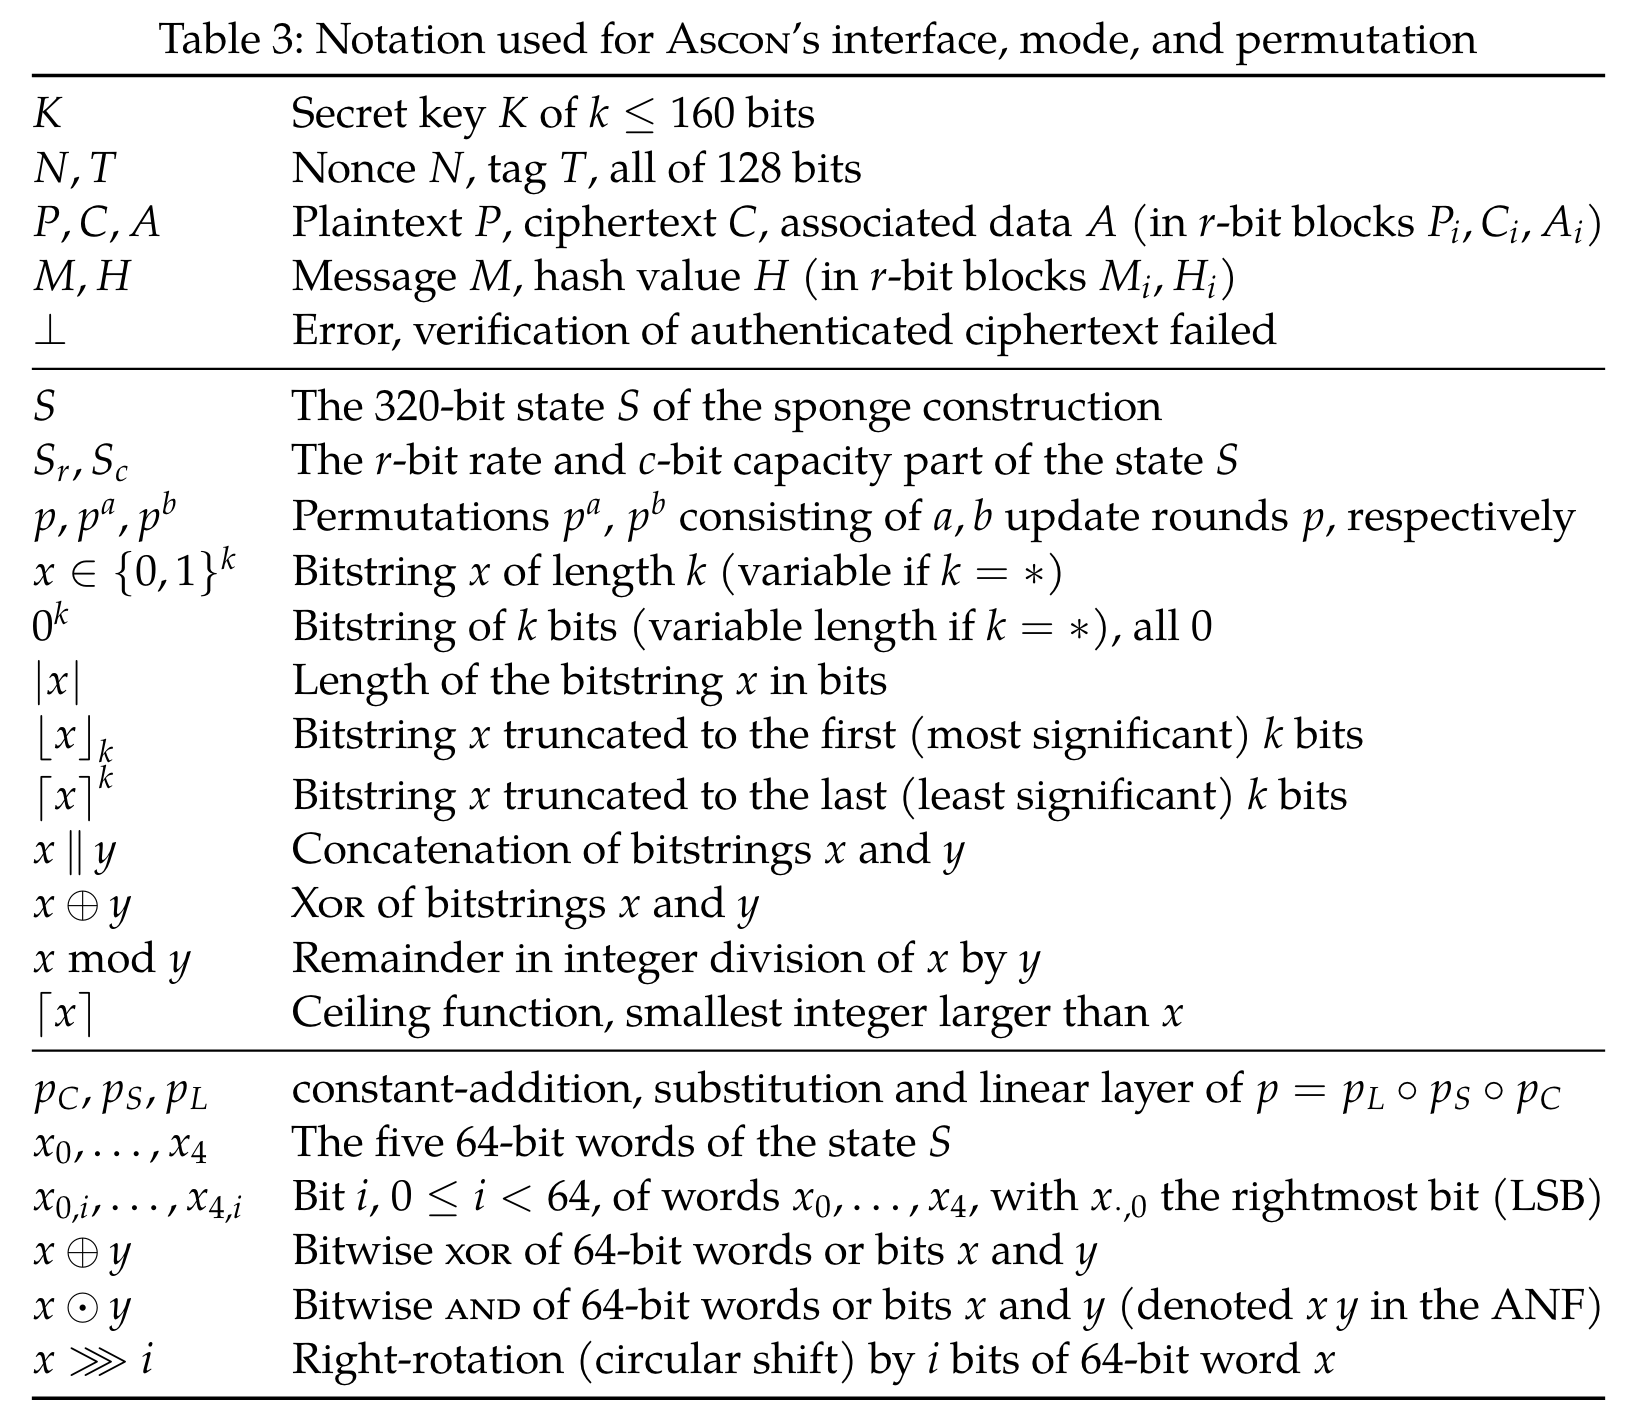
\includegraphics[width=1\textwidth]{figures/ascon-notation.png}
    \caption{Ason's Notation Table \cite{Ascon-v1.2}}
    \label{fig:ascon-notation} 
  \end{figure}

\section{Introduction}
Lightweight cryptography has emerged as a critical area of research, driven by the proliferation of resource-constrained devices such as IoT gadgets, RFID tags, and embedded systems. These devices require cryptographic solutions that are not only secure but also optimized for low power consumption, limited computational capability, and minimal memory usage. Traditional cryptographic algorithms often fall short in these environments due to their resource-intensive nature.
\newline
This paper addresses the challenges and approaches in the realm of lightweight cryptography. We explore the fundamental principles guiding the design of lightweight cryptographic algorithms and examine specific categories, including authenticated encryption, hashing, and permutations. Each section provides a comprehensive analysis of the current state-of-the-art techniques, discussing their advantages and limitations in the context of constrained environments.
\newline
Our goal is to present a detailed overview of the landscape of lightweight cryptography, highlighting recent advancements and identifying areas for future research. This study serves as a valuable resource for researchers and practitioners aiming to develop and implement efficient cryptographic solutions for the next generation of connected devices.

\section{Lightweight Cryptography}
The term lightweight cryptography refers to cryptographic algorithms that are designed to be secure even when operating in resource-restricted environments. These environments typically have limitations in terms of power, processing capabilities, memory, and even area/space. Lightweight cryptography aims to provide efficient and modernized algorithms that can operate effectively in such constrained settings.



\subsection{The Need for Lightweight Cryptography (LWC)}
Traditional cryptographic algorithms are designed to be secure, but they are often not suitable for environments with limited resources. In recent years, there has been an increasing need for lightweight cryptographic algorithms. This need arises from the growing number of devices connected to the internet. These devices are often small and have limited capabilities.
\newline
The Internet of Things (IoT) refers to a network built by interconnected devices (Figure~\ref{fig:IoT}). These devices gather data from their environment, such as a toaster with a temperature sensor or a sensor in a nuclear power plant, and exchange it with other devices in the network~\cite{chauhan2022analysis}.

\begin{figure}[h]
    \centering
    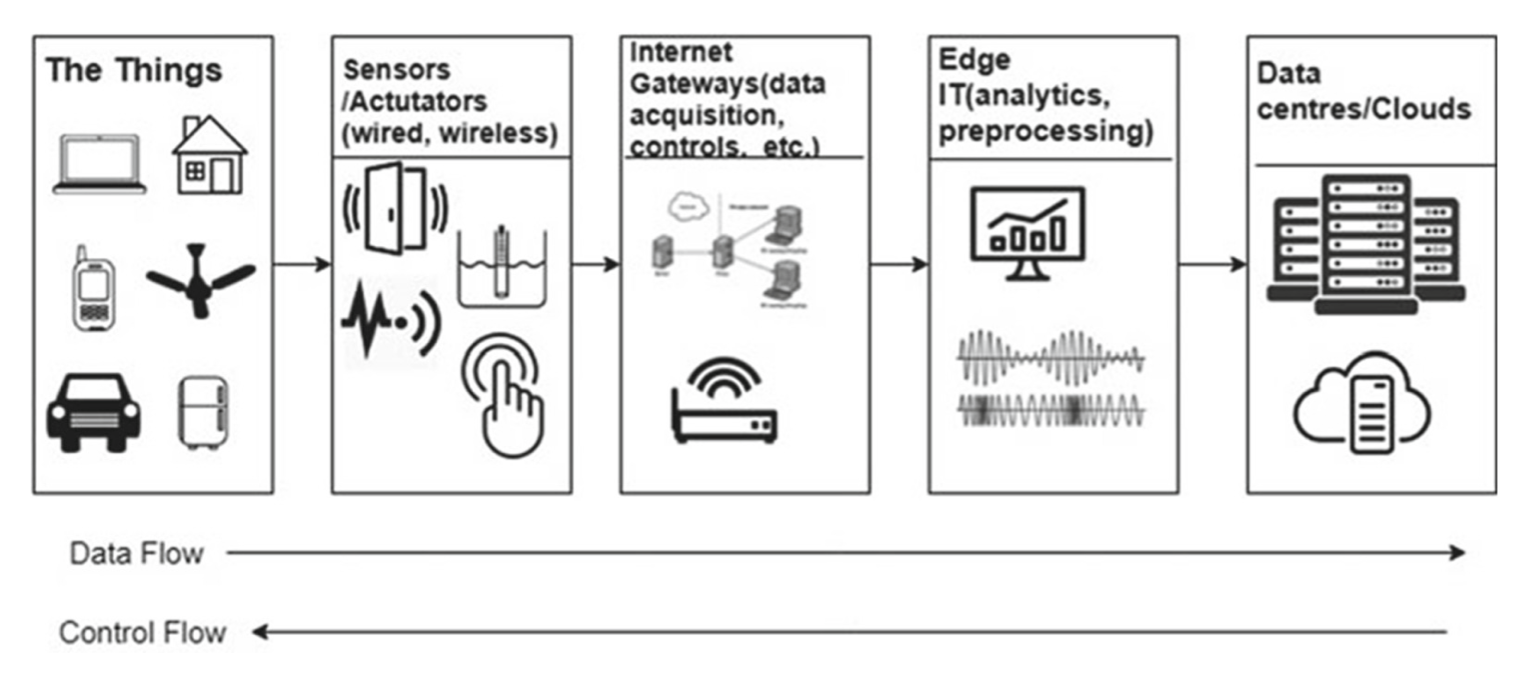
\includegraphics[width=14.0cm, height=6.0cm]{media/DesignofInternetofThings(IoT).png}
    \caption{Design of IoT}
    \label{fig:IoT}
\end{figure}

IoT devices are used in various areas and will become even more important in the future. For example, they are used in:
\begin{itemize}
    \item Smart homes for security monitoring
    \item Smart cities for traffic control and disaster management
    \item Healthcare for patient monitoring
    \item Smart grids for energy management
    \item Self-driving vehicles where cars can generate hundreds of megabytes per second
\end{itemize}
Many of these devices operate in public and sometimes inaccessible areas, making both maintenance and power supply challenging. Additionally, they are often connected over wireless networks, making them vulnerable to node tampering.

\begin{figure}[h]
    \centering
    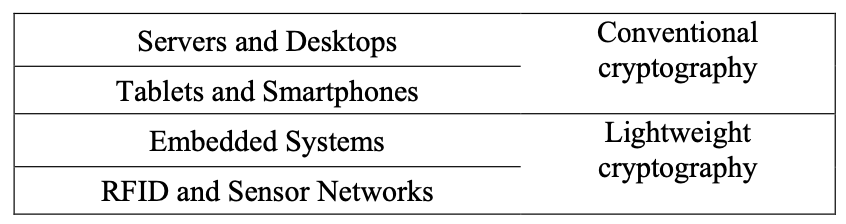
\includegraphics[width=9.0cm, height=2.5cm]{media/device_spectrum.png}
    \caption{Device Spectrum}
    \label{fig:device_spectrum}
\end{figure}

Figure~\ref{fig:device_spectrum} illustrates a rough categorization of devices based on their cryptographic requirements. More specifically, targeted devices can range from microcontrollers with 32-bit down to 4-bit CPUs. In these cases, the narrow data path and limited instruction set of the CPU architecture pose significant constraints. Executing complex cryptographic algorithms on such devices requires many more cycles, further slowing down the process due to potential battery constraints. Additionally, some controllers have as little as 16 bytes of RAM, while RFID devices are even more constrained~\cite{mckay2016report}. Therefore, it is important to have cryptographic algorithms that are secure and do not require excessive resources~\cite{IOTMarkets}~\cite{dhanda2020lightweight}.



\subsubsection{NIST's Endeavor to Standardize LWC}
While the National Institute of Standards and Technology (NIST) has standardized secure algorithms like AES, in the past, these algorithms are not suitable for use in IoT due to the diversity, scalability, and constantly changing nature of these devices~\cite{ekwueme2024lightweight}. However, NIST initiated a project in 2015 to standardize lightweight cryptographic algorithms.

In cryptography, there is always a tradeoff between performance and the required resources to complete a task at every security level.

Understanding the specific security needs of IoT devices is crucial to grasp their requirements. These needs include:

\begin{itemize}
    \setlength{\itemsep}{-5pt}
    \item \textbf{Confidentiality}: Only authorized users or systems should have access to the devices or the network.
    \item \textbf{Availability}: The required data should be available even when multiple simultaneous connections are established.
    \item \textbf{Integrity}: Manipulation of the data should be avoided.
    \item \textbf{Authentication}: Authentication is the process of verifying the identity of a user or device. Due to the diverse range of devices and protocols in IoT networks, achieving authentication and security can be  particularly challenging~\cite{dutta2019lightweight}~\cite{dhanda2020lightweight}.
\end{itemize}

Further, the metrics used to define the requirements for the process of selecting lightweight algorithms are as follows:

\begin{itemize}
    \setlength{\itemsep}{-5pt}
    \item \textbf{Security}: The security of a cipher refers to its ability to resist various types of attacks, including Side Channel Attacks. A minimum key size of at least 128 bits is necessary.
    \item \textbf{Energy consumption}: Many IoT devices run on batteries, thus it is important to minimize power consumption to ensure they can complete their tasks.
    \item \textbf{Latency}: Latency is the time it takes between starting the encryption process and producing the ciphertext. Minimizing latency is crucial for fast-running systems like interconnected cars.
    \item \textbf{Throughput}: Throughput (Kbps) can be thought of as the performance that describes the frequency at which new outputs are generated, which should be in a moderate scale for these devices.
    \item \textbf{Chip Area}: This hardware-specific metric describes the area of a chip implementation measured in gate equivalence (GE) in µm2. The need for area and the consumption of power can be correlated. Consequently, a smaller implementation area can reduce power consumption.
    \item \textbf{Memory Usage}: Efficient memory usage is essential for software applications to ensure optimal performance and resource utilization. Minimizing the amount of memory required for data storage and manipulation can reduce costs and improve scalability~\cite{mckay2016report}.
    \item \textbf{Efficiency}: The ratio between performance and resource demands. Hardware efficiency = Throughput / physical memory, Software Efficiency = Throughput / (Code Size [KB] = algorithm size).
\end{itemize}

\begin{figure}[h]
    \centering
    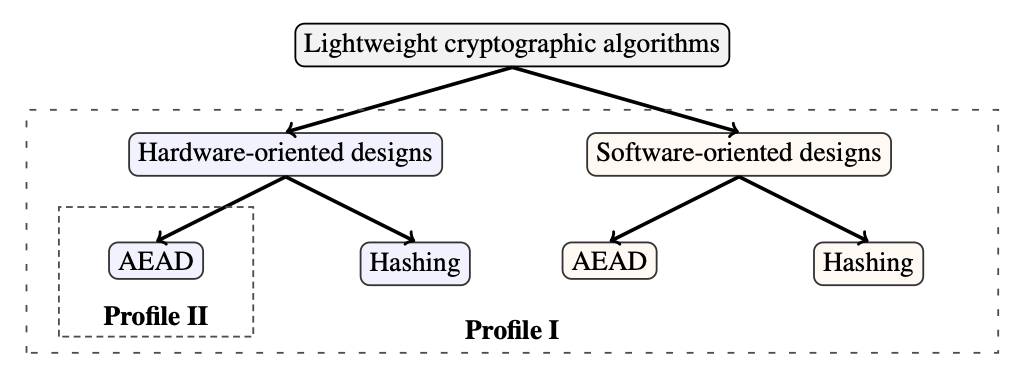
\includegraphics[width=9.0cm, height=3.5cm]{media/profiles.png}
    \caption{Profiles for lightweight cryptography applications}\label{fig:profiles}
\end{figure}

To better understand the needs and define the expectations for lightweight cryptography, NIST conducted a questionnaire among stakeholders. Based on the responses received, NIST created profiles that represent the requirements of these algorithms, which are influenced by the hardware and application areas where these algorithms are needed. The results of this questionnaire led to the creation of two profiles: Profile 1, which focuses on AEAD (Authenticated Encryption with Associated Data) and hashing for constrained software and hardware environments, and Profile 2, which focuses on AEAD for constrained hardware environments Figure~\ref{fig:profiles}. These profiles serve as guidelines for the development and evaluation of lightweight cryptographic algorithms~\cite{mckay2016report}.



\subsection{Security Issues in Lightweight Cryptography}
As mentioned above, IoT devices are openly deployed, processing, and transmitting sensitive and important data, making them high-interest targets for various attacks. Some of these attacks include Denial of Service (DoS) attacks, where the goal is to shut down the targeted system, such as a server, by overwhelming it with a high volume of data. Additionally, IoT devices with weak built-in security and low computing power (e.g., CCTV cameras and baby monitoring devices) can be injected with malware and used to execute Distributed Denial of Service (DDoS) attacks on servers~\cite{mckay2016report}~\cite{salim2020distributed}. These attacks can have severe consequences, especially in critical applications like e-Health, where a service outage could be life-threatening, or in smart cities, where an attack could disrupt the functioning of an entire city~\cite{dhanda2020lightweight}.

Crucial attacks on IoT devices include:

\begin{itemize}
    \item \textbf{Exhaustive Key Assault Attack}: Exhaustive key assault attack: This attack tries to determine the key by attempting as many keys as possible, also known as a brute force attack. Lightweight cryptography needs to ensure that it can withstand brute force attacks despite using shorter key lengths that are suitable for small devices. Cryptographic systems that use a key length of \( 2^{128} \) and higher are considered secure enough, as the theoretical attack limit is less than \( 2^{128} \) with current technology.
    \item \textbf{Table Lookup Attack}: Table lookup attack: This attack involves pre-computing the ciphertexts for all possible keys of a given length. It poses a risk for devices that use predictable or keys that are not complex enough.
    \item \textbf{Differential Attacks}: These attacks are successful when changes in plaintext result in predictable changes in ciphertext~\cite{ekwueme2024lightweight}.
    \item \textbf{Algebraic Fault Attack (AFA)}: In this case, attackers induce faults into the encryption process and use algebraic techniques to analyze these faults and ultimately recover the key. The attack involves the following steps:
    \begin{enumerate}
        \item \textbf{Fault Induction}: Faults are induced during the encryption process by manipulating physical conditions like voltage, temperature, or clock frequency of the device.
        \item \textbf{Data Collection}: The corrupted outputs are collected. Those outputs are influenced by the specific induced faults and differ from the expected results.
        \item \textbf{Equation Formulation}: A set of algebraic equations is formulated based on the differences between the expected outputs and the faulty outputs. Those equations represent the relationship between the cryptographic key (or other secret data), the input, the faulty output, and the nature of the fault.
        \item \textbf{Equation Solving}: The next step is to solve these algebraic equations for the unknowns, which typically include the secret cryptographic keys. The process of solving can be computationally intensive and involve advanced algebraic computations and special software tools.
        \item \textbf{Key Recovery}: If the equations are solved, sensitive information and the key can be extracted and used to decrypt other messages and data that have been secured with the extracted key.
    \end{enumerate}
    Since lightweight block ciphers have simpler algebraic structures than traditional ciphers, the induced faults have a bigger impact on them, and the equations can be solved easier, thus this attack can be a significant security risk. For example, if the attacker has knowledge of 24 key bits and alters two bits in the 13th round, DES can be broken with a single fault injection in 0.01 hour, resulting in 10x the speed of a brute force attack~\cite{zhang2016framework}.
    \item \textbf{Side Channel Attack (SCA)}: SCAs do not exploit the algorithm itself but the physical leakages from a cryptographic device during its normal operation. These leakages can include power consumption, electromagnetic emissions, timing information, etc. An experiment on how this is done can be seen in Figure~\ref{fig:em_measurment}, where the electromagnetic (EM) signal of two Arduino microcontrollers implementing the AES-128 algorithm is measured~\cite{pammu2016interceptive}.
    
        \begin{figure}[h]
            \centering
            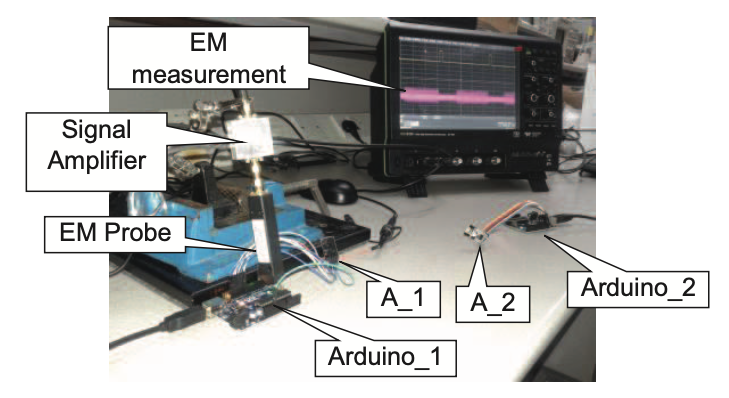
\includegraphics[width=10cm, height=4cm]{media/em_measurment.png}
            \caption{EM measurement of AES-128 based Arduino implementation}
            \label{fig:em_measurment}
        \end{figure}

    Since these devices have limited computing power and a small GE, the operations they perform, such as multiplications and additions, can be analyzed. In contrast, PCs with high computational capabilities are not as easily analyzed for patterns.
    \end{itemize}



\subsection{Mechanisms and Functionality}

Lightweight cryptography is not a separate branch of cryptography, but rather a subset of cryptographic techniques tailored to specific requirements.

Cryptography is generally divided into symmetric cryptography and asymmetric cryptography. In symmetric cryptography, the sender and receiver share the same key. It is considered a fast and secure way of encryption. The main challenge is securely exchanging the key with the communication partner. Furthermore, if the key is revealed, the encryption is compromised. 

In asymmetric encryption, each partner has one private key and one public key. The private key is known only to the owner, while the public key is revealed to the public. The private key is used to decrypt text that has been encrypted with the public key. This way, each partner can use the public key of the other to encrypt text that is meant for the other, and their own private key to decrypt text that is meant for themselves~\cite{ekwueme2024lightweight}. 

Although asymmetric cryptography is secure and solves the problem of key exchange, the keys have to be much longer than in symmetric cryptography. Thus, it is more demanding in terms of hardware resources. Since symmetric cryptography has lower demands in terms of storage, processing power, complexity, and bandwidth, it is considered the preferred method in IoT~\cite{khudoykulov2022comparison}~\cite{ekwueme2024lightweight}.

\begin{figure}[h]
    \centering
    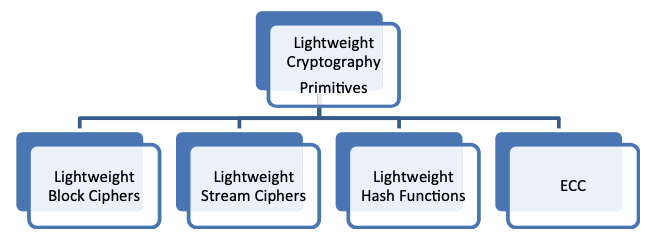
\includegraphics[width=11cm, height=4cm]{media/primitives_for_IoT.png}
    \caption{Lightweight cryptographic primitives for IoT}
    \label{fig:primitives_for_IoT}
\end{figure}


\subsubsection{Classification and Design of Lightweight Primitives}
Similar to conventional cryptography, lightweight cryptography includes four types of primitives: Lightweight Block Ciphers (LWBC), Lightweight Stream Ciphers (LWSC), Lightweight Hash Functions (LWHF), and Elliptic Curve Cryptography (ECC) (Figure~\ref{fig:primitives_for_IoT})~\cite{dhanda2020lightweight}. While stream ciphers have their uses in cryptography for IoT applications, the adaptability of block ciphers is preferred. The similarity between encryption and decryption operations in block ciphers allows for reduced resource consumption and simpler hardware and software implementations.

\textbf{Basic Block Cipher Design}
\begin{itemize}
    \item \textbf{Substitution-box (S-box)}: The S-box performs a substitution operation by taking a small block of input bits (often 4 bits) and transforming them into an output block of bits of the same size. This process, also known as confusion, introduces complexity and unpredictability between input and output bits.
    \item \textbf{Permutation-box (P-box)}: The P-box scatters the output bits of the S-box across the plaintext, ensuring that each change to an input bit influences many output bits. This step, known as diffusion, together with the S-box, makes it harder for an attacker with access to the plaintext and ciphertext to extract the key.
    \item \textbf{Rounds}: In block ciphers, the encryption and decryption processes are divided into several phases called ``rounds''.
    \item \textbf{Substitution-Permutation Network (SPN)}: This is a structure used in each round of encryption, where S-boxes and P-boxes are applied systematically. AES is probably the most popular SPN-based algorithm, with others including PRESENT and GIFT~.
    \item \textbf{The Feistel Network (FN)}: Another structure used in block ciphers is the Feistel Network, where the input block is divided into two equal parts, and during each round, only one half of the block is processed (using substitution and permutation), and then the output is combined with the other half. Some algorithms based on FN include TEA and Camellia~\cite{ekwueme2024lightweight}~\cite{chauhan2022analysis}.
\end{itemize}



\subsection{Unaddressed Needs and Introduction to Ascon}

Just in the last 10 years, Lightweight Cryptography (LWC) has gained attention from the community, thus many aspects were unaddressed in the past. Some of the research gaps for LWC primitives back in 2020 can be seen in Figure~\ref{fig:Research_gaps}~\cite{dhanda2020lightweight}.

\begin{figure}[h]
    \centering
    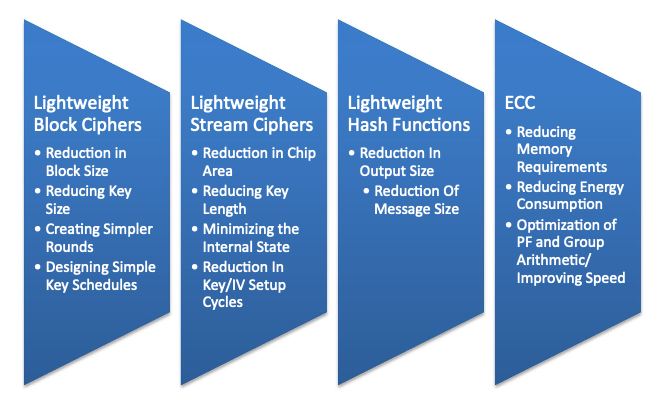
\includegraphics[width=12cm, height=7.5cm]{media/Research_gaps.png}
    \caption{Research gaps for LWC primitives}
    \label{fig:Research_gaps}
\end{figure}

NIST sets rules for Lightweight Cryptography (LWC) to improve performance and security by making specific design decisions, including:

\begin{itemize}
    \item \textbf{Smaller block sizes}: This is done to save memory, but could make the algorithms susceptible to plaintext or key recovery attacks.
    \item \textbf{Smaller key sizes}: In the past, many algorithms used keys less than 96 bits. NIST now requires at least 112 bits.
    \item \textbf{Simpler rounds}: Uses basic components to save space. For example, a 4-bit S-box in PRESENT uses only 28 GEs compared to 395 GEs for the AES S-box. Simpler designs may require more rounds to be secure.
    \item \textbf{Simpler key schedules}: Reduces memory and power needs but may increase vulnerability to certain types of attacks. Secure key functions can help prevent these.
    \item \textbf{Minimal implementations}: Only includes essential functions, which saves space and power. Some devices might only need to encrypt or decrypt, not both~\cite{mckay2016report}.
\end{itemize}

Following the evaluation of the finalists using the specified criteria, NIST has chosen the ASCON family for standardization. This group includes AEAD and hash functions, as well as extra XOFs. The design of ASCON, which is based on permutations, allows it to meet a broad range of application requirements at a low additional cost for implementing new functionalities. A detailed examination of ASCON will be the content of the following chapters~\cite{turan2021status}.



\section{Authenticated Encryption with Associated Data}
% Questions:
% what is S_r and S_c?
% What is a Nonce And Tag?
After many years of relying on traditional methods for encryption and authentication through 'generic composition,' new constructions have emerged over the past two decades. They achieved both privacy and authenticity simultaneously and often more efficiently than solutions using generic composition.
\newline
In many environments we do not only have to encrypt and authenticate the message or payload, but also wish to include auxiliary data (like the header of a network packet) which should be authenticated, but left unencrypted. \cite[Chapter 1]{Black2005}
The purpose of not encrypting but authenticating the associated data, is for router needing to be able to read the headers of packets in order to know how to properly route them. This need spurred the progress of AE schemes to allow "associated data" to be included as input. Such schemes have been termed AEAD schemes (Authenticated Encryption with Associated Data) which rely on symmetric key cryptography.\footnote[1]{\textbf{Symmetric key cryptography}, also called secret or single-key cryptography, uses the same key to both encrypt and decrypt information and is used primarily to ensure data confidentiality. In cases where the information is encrypted and decoded by the same person, there is no need to share the secret key. However, when these operations involve different people or equipment, it is necessary that the secret key be previously combined through a secure communication channel. \cite{Alencar2022Cryptography}}\cite[Chapter 1]{Black2005}
A notion which was first formalized by Rogaway \cite{10.1145/586110.586125}.

\subsection{Ascon AEAD Scheme}
In this section, we dive into the Ascon-128 scheme, which, along with Ascon-128a, has been designated as the “primary choice” for lightweight authenticated encryption in the final portfolio of the CAESAR competition. These schemes are notable for their robust security, with no known vulnerabilities. The most effective attacks target only the versions with reduced rounds—specifically, the initialization reduced to 7 out of 12 rounds—and these are still far from posing a practical threat. Notably, benchmarks have demonstrated that Ascon excels in efficiency, particularly for short messages, confirming its status as a state-of-the-art lightweight encryption method. \cite[Chapter 1]{Ascon-v1.2}


\subsection{Authenticated Encryption $E_{k,r,a,b}$}
The encryption procedure $E_{k,r,a,b}$ takes the following inputs:
\begin{itemize}
    \item Secret key $K$ with $k$ bits.
    \item Nonce (public message number) $N$ with 128 bits. \footnote[2]{\textbf{Nonce:} A random or non-repeating unique value that is included, usually for the purpose of protecting against replay attacks. \cite[Page 200]{rfc4949}}
    \item Associated data $A$ of arbitrary length. (f.e. the header of a networkpacket)
    \item Plaintext $P$ of arbitrary length. (the payload)
\end{itemize}
It produces an output consisting of the authenticated ciphertext $C$ of exactly the same length as the plaintext $P$ plus an authentication tag $T$ of size 128 bits, which authenticates both the associated data and the encrypted message:

\[
E_{k,r,a,b}(K,N,A,P) = (C,T)
\]
Here, $A$ is not encrypted but authenticated. 
The recommended parameterset for Ascon-128 is $E_{128,64,16,6}$ and for Ascon-128a $b$ is 8. \cite[Chapter 2.2]{Ascon-v1.2} \newline
To reduce the effort of implementing the algorithm on new target platforms, Ason is natively defined on 64-bit words using only bitwise operations and Boolean functions. \cite[Chapter 4.1]{Ascon-v1.2}

\subsection{Decryption and Verification $D_{k,r,a,b}$}
The decryption and verification procedure $D_{k,r,a,b}$ takes the following inputs:
\begin{itemize}
    \item Key $K$.
    \item Nonce $N$.
    \item Associated data $A$.
    \item Ciphertext $C$.
    \item Tag $T$.
\end{itemize}
It outputs either the plaintext $P$ if the verification of the tag is correct, or an error $\bot$ if the verification of the tag fails:
\[
D_{k,r,a,b}(K,N,A,C,T) \in \{P, \bot\}
\]
\cite{Ascon-v1.2}

\subsection{Algorithm} % TODO: Find duplex mode citation
\sloppy
Ascons approach for authenticated encrytion is based on duplex modes\footnote[3]{\textbf{The duplex construction} uses a fixed permutation to process input and output simultaneously, inheriting security from the sponge construction and enabling efficient authenticated encryption with just one permutation call per message block, where input blocks encode data and keys, and output blocks provide encryption and authentication. \cite{10.1007/978-3-642-28496-0_19}} like MonkeyDuplex, but contrary to other sponge-based authenticated encryption schemes, Ascon uses stronger keyed initialization and keyed finalization phases. This makes sure that if an attacker manages to recover the internal state during data processing (f.e. with side-channel attacks), the attacker is not directly able to recover the secret key. \cite[Chapter 5.1]{Ascon-v1.2}
The encryption and decryption operations are depicted in Figure 2. \cite{Ascon-v1.2}
\begin{figure}[H]
    \centering
    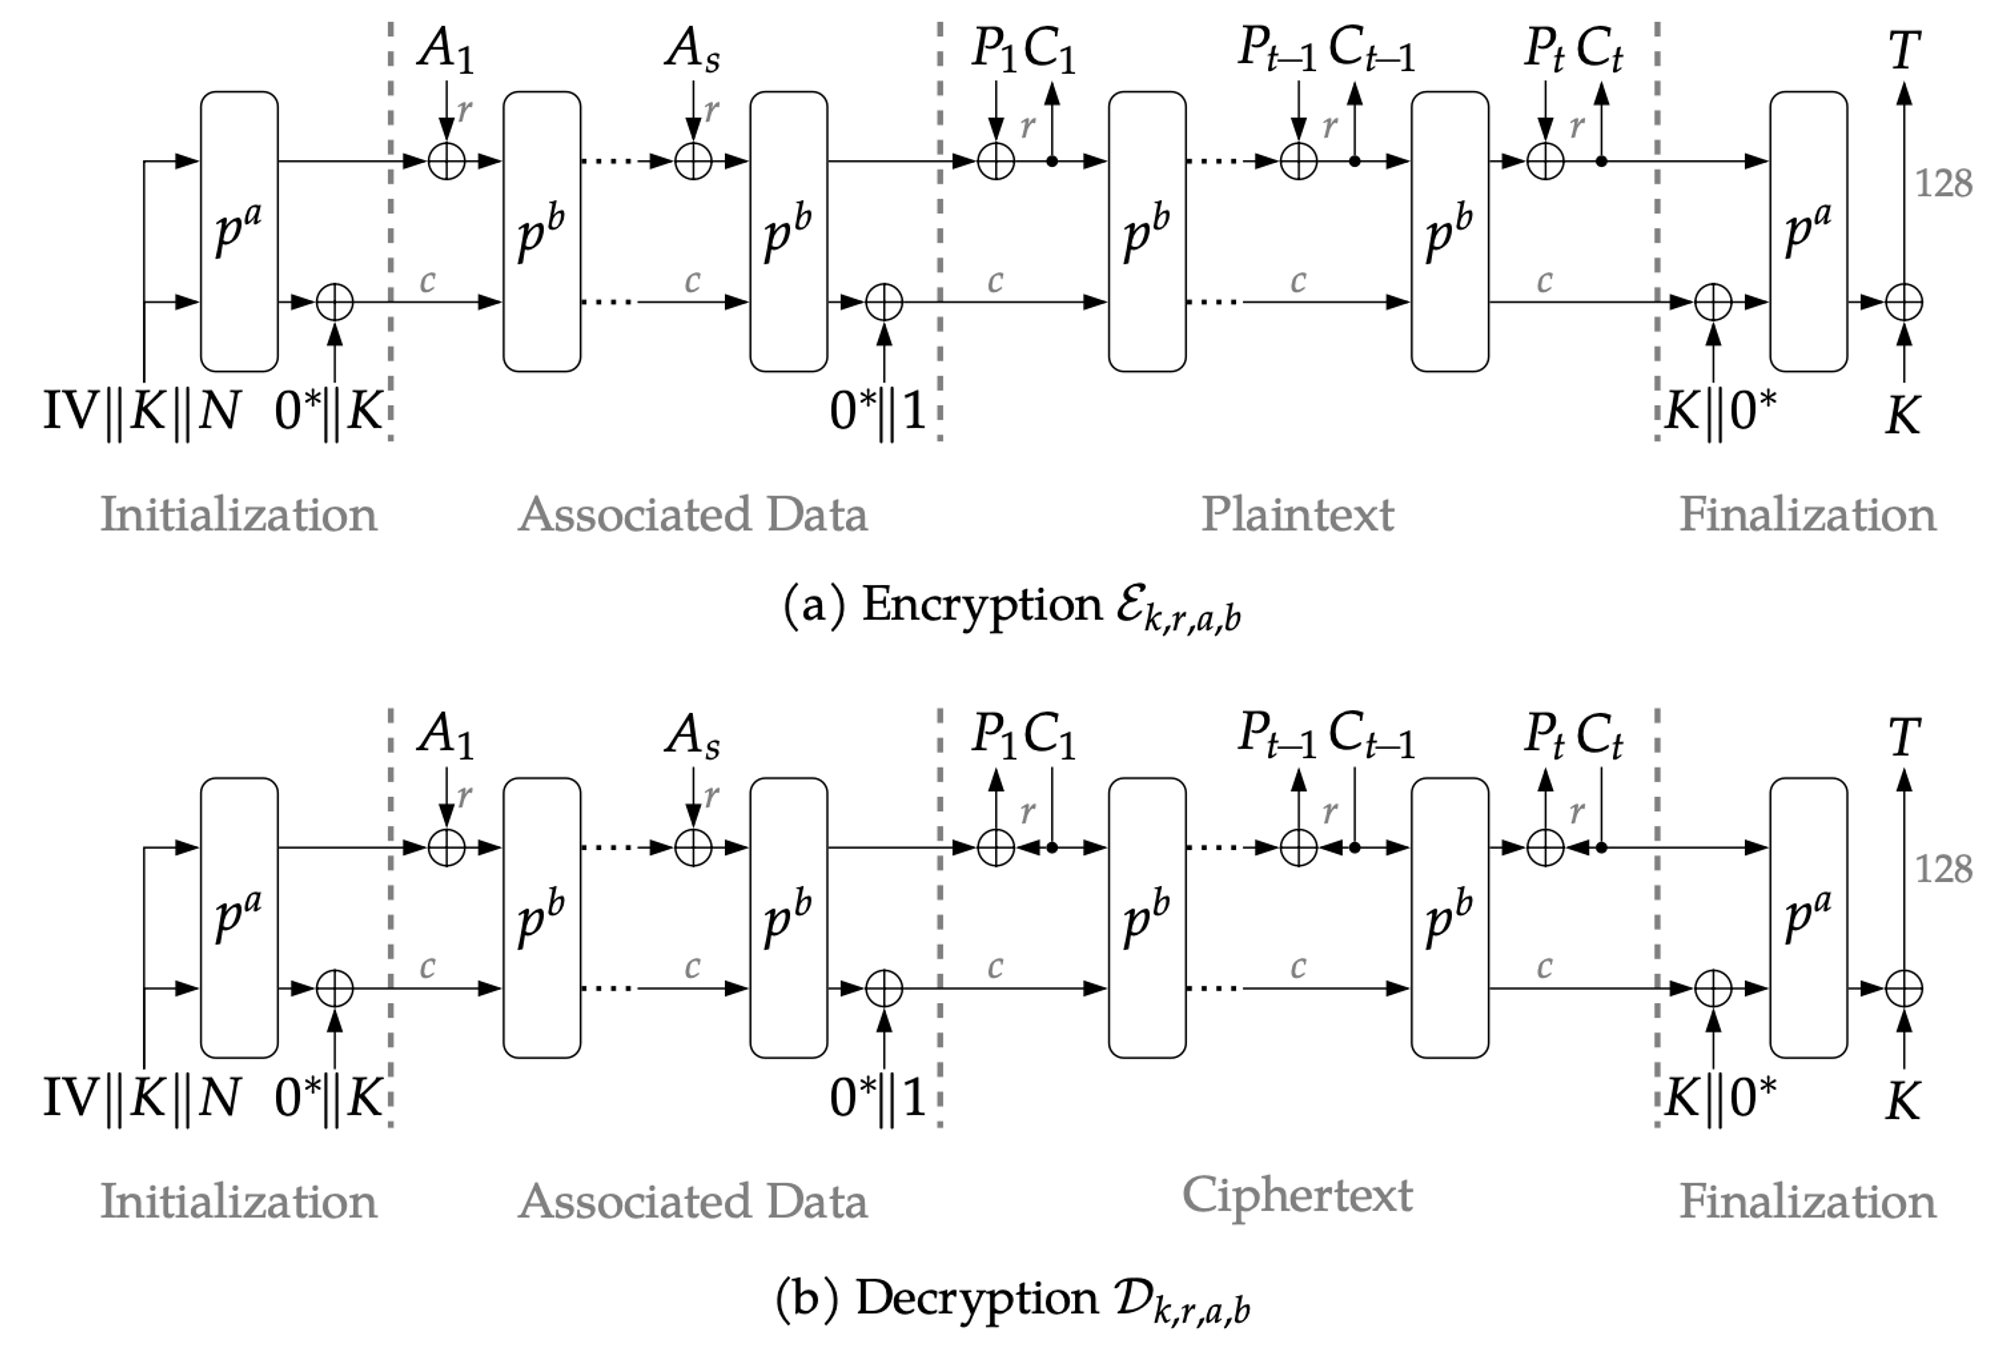
\includegraphics[width=1\textwidth]{figures/aead-algorithm.png}
    \caption{Ascon's mode of operation \cite{Ascon-v1.2}}
    \label{fig:aead-algorithm}
\end{figure}
\subsubsection{Initialization}

"The 320-bit initial state of Ascon is formed by [concatenating] the secret key K of k bits and nonce N of 128 bits, as well as an IV specifying the algorithm (including the key size k, the rate r, the initialization and finalization round number a, and the intermediate round number b, each written as an 8-bit integer)", followed by padding of zeros for the required length.
$$S \leftarrow k || r || a || b || 0^{160-k} || K || N $$
In the Initialization $a$ rounds of the permutation $p$ is applied to the initial state. After that, the resulting state is XORed with a modified version of the secret key $K$ which is prepended with a series of $320-k$ zeros to pad it to the size of 320 bits. \cite{Ascon-v1.2}
$$S \leftarrow p^a(S) \oplus (0^{320-k} || K)$$
% This step is needed to... % finish this
\subsubsection{Processing Associated Data}
If there is associated data, it will first be preprocessed for absorbtion into blocks of $r$ bits which will be appended by a single $1$ and the smallest number of zeros to obtain a multiple of $r$ and then split again in $s$ blocks of $r$ bits. If there is no associated data, no padding is apllied and $s=0$.
\sloppy
The associated data $A$ is then absorbed into the state.
\[
S \leftarrow p^b((S_r \oplus A_i) || S_c),\ \ 1 \leq i \leq s
\]
After all associated data is absorbed, a domain separation constant is added to differentiate the processing of associated data from the encryption of the payload. \cite[Chapter 2.4.2]{Ascon-v1.2}
$$S \leftarrow S \oplus (0^{319} || 1)$$

\subsubsection{Processing Plaintext/Ciphertext}
As for the payload it is also processed into blocks the same way. 
$$P_1, \dots , P_t \leftarrow \text{ r-bit blocks of } P || 1 || 0^{r-1-(|P| mod\ r)}$$
The addition of $0^{319} \Vert 1$ domain seperation is to prevent attack that change the role of plaintext and associated data blocks. In case of an imcomplete plaintext block with no associated data, the two initialization and finalization calls are sufficient without an intermediate round transformation $p^b$. This prevents that key additions between the two applications cancel each other out. In this case they are added to different parts of the capacity port $S_c$ os the state. \cite[Chapter 5.1.1]{Ascon-v1.2} \newline
For encryption each padded plaintext block $P_i$ is XORed to the first $r$ bits $S_r$ of the state $S$ and for each block except the last one is it is transformed by the permutation $p^b$% why???
$$C_i \leftarrow S_r \oplus P_i$$
$$
s \leftarrow \begin{cases} 
    p^b(C_i \parallel S_c) & \text{if } 1 \leq i < t \\
    C_i \parallel S_c & \text{if } 1 \leq i = t
    \end{cases}
$$
The last remaining block $C_t$ the padding is removed. This ensures that the decrypted plaintext matches the original plaintext exactly, without any additional padding bytes affecting the integrity of the data.
$$\tilde{C}_t \leftarrow \lfloor C_t \rfloor_{|P| \text{ mod } r}$$
\newline
To decrypt the ciphertext back the its original, each ciphertextblock except the last one is being XORed with the first $r$ bits $S_r$ of the internal state, which then has to be replaced by $C_i$ and then transformed by the $b$-round permutation $p^b$:
$$ P_i\leftarrow S_r \oplus C_i $$
$$ S \leftarrow (S_r \oplus (\tilde P_t || 1 || 0^{r-1-l})) || S_c $$
For the remaining truncated ciphertextblock $\tilde C_t\ with\ 0 \leq l \le r$ bits, the procedure differs:
$$\tilde{P}_t \leftarrow \lfloor S_r \rfloor_\ell \oplus \tilde{C}_t$$
$$S \leftarrow (S_r \oplus (\tilde P_t || 1 || 0^{r-1-l})) || S_c$$
\cite{Ascon-v1.2}
\subsubsection{Finalization}
The Finalization step, is genereting the tag which is important for \dots
The secret Key $K$ is first XORed to the internal state which then is transformed by the permutation $p^a$ using $a$. The tag $T$ consists of the last 128 bits of the state XORed with the last 128 bits of the key $K$: %why last 128 bits isnt the key exactly that long?
$$S \leftarrow p^a(S \oplus (0^r || K || 0^{c-k}))$$
$$ T \leftarrow \lceil S  \rceil^{128} \oplus \lceil K \rceil^{128}$$
The encryption procedure is returning the tag $T$ together with the ciphertext $C_1||...||\tilde C_t$ and the decription procedure is just returning the plaintext (payload) if the calculated tag value matches the received tag value $T$. \cite{Ascon-v1.2}

\subsection{Principles Behind Ascon's Cryptographic Techniques}
\dots



\section{Hashing}
Hash functions are a cryptographic primitive with many useful applications in computer science. Hashes are used to verify data integrity, and play an important role in entity authenticity and digital signature schemes. They can be used for cryptographic key derivation, key and pseudorandom number generation; moreover, blockchain principle is built entirely on hashing. Aforementioned applications are also prevalent in the context of lightweight cryptography \cite{lightHashTrends}. The following chapter is going to introduce a reader to hash functions in general and present the hashing design of the ASCON family.

% First, we will look at the theoretical requirements for the hash functions, and then proceed with the practical
\subsection{Hash function and its requirements}
Simply put, a cryptographic hash function $ \mX: \{0, 1\}^* \rightarrow \{0,1\}^{l} $ takes an input bitstring $x$ of arbitrary length and produces a short bitstring output $y$ of fixed length $l$, also called a digest, or a hash value. Such mapping allows us to identify any $x$ with some shorter $y$. 

\subsubsection{Collision resistance}
Theoretically, because the domain of possible inputs is larger than of the range of the hash function, and since the mapping is surjective, there is an infinite amount of possible messages, such that their hash values are identical. Since $ |\{0,1\}^*| $ is infinite and $ |\{0,1\}^l| = 2^l $, by the pigeonhole principle, there exist at least two bitstrings $ x_1, x_2 \in \{0,1\}^* $, with $ x_1 \neq x_2 $, such that $ \mX(x_1) = \mX(x_2) $. This equality of digests of two or more input values is called a collision \cite{knospeCourseCryptography2019}.

Practically, it is very hard to find such collisions. The ``hardness'' is described by the theoretical amount of needed prompts to a hash function to acquire at least one of such events, and the requirement for a low probability of collision is called a \textit{collision resistance}. By simply trying out 
\[
\mX(x_1), \mX(x_2), \mX(x_3), \ldots
\]
and comparing each next hash value with previous ones, eventually, an attacker is going to stumble upon a collision. In order for $x_1, x_2, x_3, \ldots$ not to share a matching hash, each of these probed inputs must not yield a match with any other probed input. And since a number of possible hashes is finite, the probability of not having a single collision pair decreases exponentially with each new input. To find an expected amount of trials needed for a 50\% chance of getting a match, we can apply an approximation for the Birthday Problem: 
\[n\approx \sqrt{2d\cdot p}, \]
where $d$ is the number of possible outcomes, and $p$ is a desired probability. This yields us a $\sqrt{2^l} = 2^{l/2}$. For example, if a hash function produces a 256-bit digest, one has to probe $2^{128}$ number of inputs to merely have a 50\% chance of getting a pair of matching hashes, which is sufficiently infeasible under our current compute capabilities; moreover, one has to have a tremendous storage of at least $2^{133}$ bytes ($10^{25}$ petabytes) for such an endeavor.

\subsubsection{(Second-) preimage resistance}
If we would like to use hash functions as a reliable means to verify an integrity or authenticity of important information, two more requirements arise. One would not like, if an attacker, knowing the hash value $y$, easily guessed or picked a suitable input $\hat{x}$, such that $\mX(\hat{x}) = y$, because he could perfectly disguise the matching $\hat{x}$ as a valid piece of data, or worse, find out the true input. The property that allows to withstand such attacks is called \textit{one-wayness} or \textit{preimage resistance}, the $x$ being a preimage of $y$. The second undesirable situation is when an adversary can, for a given input $x$ that he knows, find such $x^\prime$ that $\mX(x^\prime) = \mX(x)$ and $x^\prime \neq x$. This means that we would like a hash function to ensure that it is hard to find not just any collision, but a specific one for a given input. This property is called a \textit{second-preimage resistance}. Both requirements yield a need to test $2^{l}$ number of inputs to break them, if a hash function is ideally constructed \cite{cryptmadesimple}.

\subsubsection{Ideal hash function}
An ideal hash function is said to be following a \textit{random oracle model}, in which a random oracle samples and outputs hash values from a random uniform distribution each time a new input is fed. If a random oracle again receives an input that was given in the past, it yields the same hash as one he returned the first time for this input. The design of the hash functions is tested against the ideal random oracle model by theoretical proofs and is aimed to be sufficiently close to, or \textit{indifferentiable} from, it.

\subsection{Hash constructions}
The first widely used idea to bring an infinite domain to a finite range of hash values is to use a \textit{compression function} $f$. Message $M$ is first padded and split into chunks of equal length $M=x_1||x_2||x_3||\ldots||x_n$. A compression function then takes in a first input chunk with the initial state $S$. The previous output of the function and the next chunk of a message are then fed to the same function again, sequentially, until the message is fully expended. The end return is a hash value. This approach is called a \textit{Merkle-Damgård transform} \cite{coronMerkleDamgardRevisitedHow2005}. Its working is depicted schematically on the Figure \ref{fig:merkle}. SHA-1 and SHA-2 standard hashing algorithms were designed as Merkle-Damgård hash functions, the SHA-1 being now deprecated for discovered security flaws. In 2017, \cite{firstcollision} found the first ever collision for SHA-1.

\begin{figure}[H]
    \centering
        \tikzset{every picture/.style={line width=0.75pt}} %set default line width to 0.75pt        

        \begin{tikzpicture}[x=0.75pt,y=0.75pt,yscale=-1,xscale=1]
        %uncomment if require: \path (0,235); %set diagram left start at 0, and has height of 235
        
        %Shape: Trapezoid [id:dp989820392477355] 
        \draw   (82.75,62.7) -- (114.25,72.15) -- (114.25,126.76) -- (82.75,136.21) -- cycle ;
        
        %Straight Lines [id:da9136570431817581] 
        \draw    (39.9,98.4) -- (78.65,98.41) ;
        \draw [shift={(80.65,98.41)}, rotate = 180] [fill={rgb, 255:red, 0; green, 0; blue, 0 }  ][line width=0.08]  [draw opacity=0] (8.4,-2.1) -- (0,0) -- (8.4,2.1) -- cycle    ;
        %Straight Lines [id:da22262592186104624] 
        \draw    (61.75,31.19) -- (61.75,83.7) -- (78.65,83.7) ;
        \draw [shift={(80.65,83.7)}, rotate = 180] [fill={rgb, 255:red, 0; green, 0; blue, 0 }  ][line width=0.08]  [draw opacity=0] (8.4,-2.1) -- (0,0) -- (8.4,2.1) -- cycle    ;
        %Shape: Trapezoid [id:dp8730607411910694] 
        \draw   (178.11,62.74) -- (209.61,72.19) -- (209.61,126.8) -- (178.11,136.25) -- cycle ;
        
        %Straight Lines [id:da7073511289859868] 
        \draw    (114.25,98.44) -- (174,98.45) ;
        \draw [shift={(176,98.45)}, rotate = 180] [fill={rgb, 255:red, 0; green, 0; blue, 0 }  ][line width=0.08]  [draw opacity=0] (8.4,-2.1) -- (0,0) -- (8.4,2.1) -- cycle    ;
        %Straight Lines [id:da8571759413814846] 
        \draw    (157.1,31.23) -- (157.1,83.74) -- (174,83.74) ;
        \draw [shift={(176,83.74)}, rotate = 180] [fill={rgb, 255:red, 0; green, 0; blue, 0 }  ][line width=0.08]  [draw opacity=0] (8.4,-2.1) -- (0,0) -- (8.4,2.1) -- cycle    ;
        
        %Shape: Trapezoid [id:dp010143672535839032] 
        \draw   (273.46,62.74) -- (304.97,72.19) -- (304.97,126.8) -- (273.46,136.25) -- cycle ;
        
        %Straight Lines [id:da15113595456398543] 
        \draw    (209.61,98.44) -- (269.36,98.45) ;
        \draw [shift={(271.36,98.45)}, rotate = 180] [fill={rgb, 255:red, 0; green, 0; blue, 0 }  ][line width=0.08]  [draw opacity=0] (8.4,-2.1) -- (0,0) -- (8.4,2.1) -- cycle    ;
        %Straight Lines [id:da9161491017393608] 
        \draw    (252.46,31.23) -- (252.46,83.74) -- (269.36,83.74) ;
        \draw [shift={(271.36,83.74)}, rotate = 180] [fill={rgb, 255:red, 0; green, 0; blue, 0 }  ][line width=0.08]  [draw opacity=0] (8.4,-2.1) -- (0,0) -- (8.4,2.1) -- cycle    ;
        
        %Shape: Trapezoid [id:dp04826586579594827] 
        \draw   (397.94,62.74) -- (429.44,72.19) -- (429.44,126.8) -- (397.94,136.25) -- cycle ;
        
        %Straight Lines [id:da5983989156297147] 
        \draw    (363.81,98.44) -- (393.84,98.45) ;
        \draw [shift={(395.84,98.45)}, rotate = 180.01] [fill={rgb, 255:red, 0; green, 0; blue, 0 }  ][line width=0.08]  [draw opacity=0] (8.4,-2.1) -- (0,0) -- (8.4,2.1) -- cycle    ;
        %Straight Lines [id:da1340107169372431] 
        \draw    (376.93,31.23) -- (376.93,83.74) -- (393.84,83.74) ;
        \draw [shift={(395.84,83.74)}, rotate = 180] [fill={rgb, 255:red, 0; green, 0; blue, 0 }  ][line width=0.08]  [draw opacity=0] (8.4,-2.1) -- (0,0) -- (8.4,2.1) -- cycle    ;
        %Straight Lines [id:da7846820892857251] 
        \draw    (429.44,98.44) -- (489.19,98.45) ;
        \draw [shift={(491.19,98.45)}, rotate = 180] [fill={rgb, 255:red, 0; green, 0; blue, 0 }  ][line width=0.08]  [draw opacity=0] (8.4,-2.1) -- (0,0) -- (8.4,2.1) -- cycle    ;
        %Straight Lines [id:da02924524891297775] 
        \draw    (305.18,98.4) -- (335.21,98.41) ;
        \draw [shift={(337.21,98.41)}, rotate = 180.01] [fill={rgb, 255:red, 0; green, 0; blue, 0 }  ][line width=0.08]  [draw opacity=0] (8.4,-2.1) -- (0,0) -- (8.4,2.1) -- cycle    ;

        % Text Node
        \draw (92.5,91.85) node [anchor=north west][inner sep=0.75pt]    {$f$};
        % Text Node
        \draw (187.86,91.89) node [anchor=north west][inner sep=0.75pt]    {$f$};
        % Text Node
        \draw (158.15,17.85) node    {$x_{2}$};
        % Text Node
        \draw (253.51,17.85) node    {$x_{3}$};
        % Text Node
        \draw (283.21,91.89) node [anchor=north west][inner sep=0.75pt]    {$f$};
        % Text Node
        \draw (407.69,91.89) node [anchor=north west][inner sep=0.75pt]    {$f$};
        % Text Node
        \draw (32.55,99) node    {$s$};
        % Text Node
        \draw (377.98,17.85) node    {$x_{n}$};
        % Text Node
        \draw (350.54,96.0) node    {$\ldots$};
        % Text Node
        \draw (127.31,86.72) node    {$s_{1}$};
        % Text Node
        \draw (221.31,86.7) node    {$s_{2}$};
        % Text Node
        \draw (316.7,86.7) node    {$s_{3}$};
        % Text Node
        \draw (444.31,86.7) node    {$s_{n}$};
        % Text Node
        \draw (500,98.4) node    {$H$};
        % Text Node
        \draw (62.8,17.81) node    {$x_{1}$};
        \end{tikzpicture}
    \caption{The Merkle-Damgård construction.}
    \label{fig:merkle}
\end{figure}
In a Merkle-Damgård hash function, the \textit{internal state} is fully exposed, reflecting the hash of the input. If attacker knows the hash, he knows the final state of the compression function and can ``resume'' the calculation further with an appended message, producing a valid hash. This is known as a \textit{length extension attack} on hash \cite{knospeCourseCryptography2019}.

A second architecture eliminates the length extension attack by never revealing the full internal state. This also conveniently allows for yielding an arbitrary length hash value. Such useful features are achieved by introducing a much larger internal state, allowing chunks of a message to be ``absorbed'' into the state, having a permutation function, and releasing a hash from the state also only chunk by chunk. This configuration is called a \textit{sponge construction} \cite{guido_b_d_michaël_p_2011}, and ASCON hashing adopts this particular mode of operation \cite{ascon_specification}.

\begin{figure}[H]
    \centering
    \begin{tikzpicture}
        \SpongeInitInner{$\text{IV} \| 0^c\hskip-10pt$}{$p^a$}
        \draw (P.south) +(0,-1) node[spongephase] (phase) {Initialization\phantom{p}\qquad\null};
        \SpongeStep\SpongePhaseSep
    
        \SpongeAbsorb{$M_1$}{$p^b$}{$r$}{$c$}
        \SpongeEtc
        \SpongeAbsorb{$M_{s-1}$}{$p^b$}{$r$}{$c$}
        \draw (x|-phase) node[spongephase] {Absorb Message};
        \SpongeXorOuter{$M_s$}{$r$}{$c$}
        \SpongeStep\SpongePhaseSep\SpongeStep
        \SpongePermute{$p^a$}
    
        \SpongeSqueeze{$H_1$}{$p^b$}{$r$}{$c$}
        \SpongeEtc
        \SpongeSqueeze{$H_{\lceil \ell/r \rceil}$}{$p^b$}{$r$}{$c$}
        \draw (x|-phase) node[spongephase] {Squeeze Hash\qquad\null};
        \SpongeSkip
        \SpongeEtc
    \end{tikzpicture}
  \caption{The sponge construction of ASCON.}
%   \label{fig:sponge}
\end{figure}
A sponge function is made of three components: a state memory $S$ containing ${r+c}$ bits, a permutation function $p: \left\{0,1\right\}^{r+c} \rightarrow \left\{0,1\right\}^{r+c}$ and a padding function $P$:

\begin{itemize}
  \item $S$ is divided into two parts: the $r$-bit \textit{rate} $S_r$ and the $c$-bit \textit{capacity}~$S_c$. The rate is the part of the state that is XORed with the input message, while the capacity is the part that stays hidden. Both rate and capacity are then being permuted together by the function $p$;
  \item $p$ produces a pseudo random permutation of the $2^{r+c}$ possible states, details of which are shown in the next chapter;
  \item $P$ is a function that pads the input message to a multiple of $r$.
\end{itemize}

The sponge function is performed iteratively in two phases: the \textbf{absorbing phase} and the \textbf{squeezing phase}. During preprocessing, an input message is padded and cut into $r$ bit blocks $M_1||M_2||\ldots||M_s$. In the absorbing phase, blocks of the input message are mixed with $S_r$ using per bit XOR operation. Then a result is concatenated with the capacity and passed through $p$ to become a new state again:
\begin{equation}
    S \leftarrow p((S_r \oplus M_i)~||~S_c)~\text{for}~1 \leq i \leq s. \notag
\end{equation}


In the squeezing phase, the finalizing permutation is applied to $S$ and the first leftmost $r$ bits of the state are retrieved. This process is repeated until the outputs $H_1||H_2||\ldots||H_t$ reach the desired length $\ell$.
\[
    H_i \leftarrow S_r
\]
\[
    S \leftarrow p(S)
\]

The last $c$ bits are neither XORed nor directly output, and thus the full state never leaves the hash function.

\subsection{ASCON hashing}
ASCON's hash has an internal state of 320 bits, with 64-bit rate and 256-bit capacity. Authors provide four configurations: \textsc{Ascon-Hash, Ascon-Hasha, Ascon-Xof}, and \textsc{Ascon-Xofa}. The \textit{initialization vector} IV for each configuration is set as follows:
\[
\text{IV}_{h,r,a,b} \leftarrow 0^8 \parallel r \parallel a \parallel a - b \parallel h =
\begin{cases}
    00||40||0c||00||00000100 & \text{for }\textsc{Ascon-Hash} \\
    00||40||0c||04||00000100 & \text{for }\textsc{Ascon-Hasha} \\
    00||40||0c||00||00000000 & \text{for }\textsc{Ascon-Xof} \\
    00||40||0c||04||00000000 & \text{for }\textsc{Ascon-Xofa} \\
\end{cases},
\]
where $r$ is a rate, $a$ and $b$ are rounds of permutations (discussed in the next chapter), and $h$ is the desired output length. With $h=0$, for \textsc{Ascon-Xof} and \textsc{Ascon-Xofa}, the output length is unlimited. Then, the initial state is:
\[
S \leftarrow \text{IV}_{h,r,a,b} \parallel 0^{256}
\]

The configuration design of the hashes allow for 128-bit security for collision resistance and (second-) preimage resistance. This is derived from the fact that an attacker would need to guess the right capacity in order to get the full state that maps to the same input. Researchers found that a complexity for such an endeavor is $2^{c/2}$ \cite{bertoniIndifferentiabilitySpongeConstruction2008}, which is $2^{128}$ in case of the ASCON.
\section{Permutation}
\subsection{Introduction}

Permutation is a fundamental concept in cryptography. It is used in various cryptographic algorithms such as block ciphers, hash functions, and stream ciphers. A permutation is a bijective mapping from a set to itself. While it is a simple operation, it is actually one of the most important concepts used within the ASCON family. \par


\subsection{The sponge construction}

An interesting application of permutation in cryptography is the \textbf{sponge construction}. It relies on a fixed-length permutation and a padding rule to create a sponge function that can map variable-length input to variable-length output. \cite{keccak_team} \par 


\begin{figure}[htbp]
  \centering
  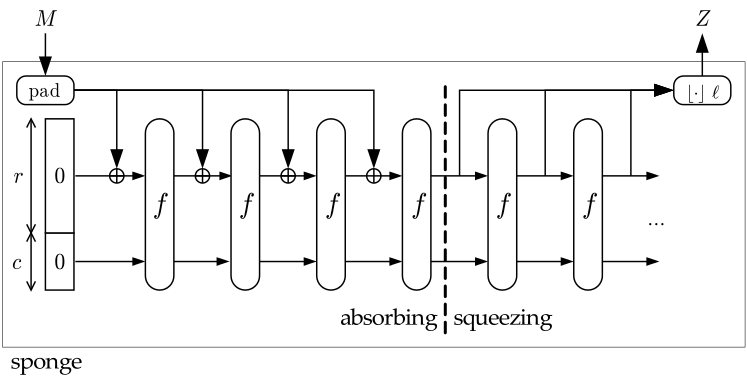
\includegraphics[width=0.5\textwidth]{images/Sponge-150.png}
  \caption{The sponge construction.}
  \label{fig:sponge}
\end{figure}

\noindent A sponge function is made up of three components: a state memory $S$ containing $b$ bits, a function $f: \left\{0,1\right\}^b \rightarrow \left\{0,1\right\}^b$ and a padding function $P$.  \cite{keccak_team,sponge_function_2023}

\begin{itemize}
  \item $S$ is divided into two parts: the rate $r$ and the capacity $c$. The rate is the part of the state that is XORed with the input message, while the capacity is the part that is not. The capacity is also the part that is permuted by the function $f$
  \item $f$ produces a pseudo random permutation of the $2^b$ possible states
  \item $P$ is a function that pads the input message to a multiple of $r$
\end{itemize}

The sponge function is performed iteratively in two phases: the \textbf{absorbing phase} and the \textbf{squeezing phase}. The padded input $M$ which is cut into $r$ bit blocks. In the absorbing phase, chunks of the input message are mixed at the beginning of the buffer using XOR operations. This can be seen in Figure \ref{fig:sponge} with the operation $r \oplus P_i$. At each step, this new buffer is again passed through $f$ causing a small amount of data to be "absorbed" into the semi-randomised buffer. \cite{keccak_team, sponge_function_2023,DBLP:journals/joc/DobraunigEMS21} \par 

In the squeezing phase, the buffer is read out in chunks of the desired output length. This is done by applying $f$ to the buffer and outputting the first $r$ bits of the result. This process is repeated until the output $Z$ with the desired length $\ell$ is reached. \cite{keccak_team,sponge_function_2023,DBLP:journals/joc/DobraunigEMS21} \par 

The last $c$ bits are neither XORed nor directly output. \par 

\subsection{The duplex construction}

\begin{figure}[htbp]
  \centering
  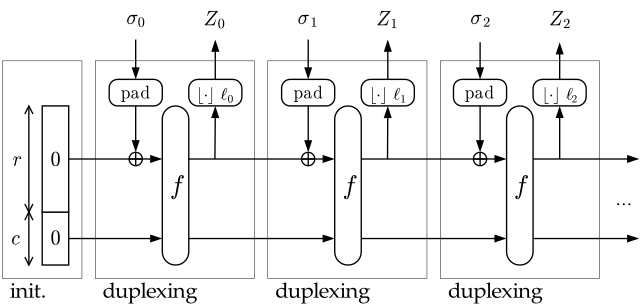
\includegraphics[width=0.5\textwidth]{images/Duplex-150.png}
  \caption{The duplex construction.}
  \label{fig:duplex}
\end{figure}

An alternation of the sponge construction is the \textbf{duplex construction}. Permutation function $f$, padding function $P$ and parameter bitrate $r$ are also used in the duplex construction, while $\sigma$ is the input string and $\ell$ is the requested number of bits. \cite{keccak_team,sponge_function_2023,guido_b_d_michaël_p_2011} \par 

While the sponge function is stateless between calls, the duplex version alternates between absorbing data into the state and squeezing data out of the state, where the output depends on all the previous inputs. \cite{guido_b_d_michaël_p_2011,cryptoeprint:2023/796} During the absorption phase, input data is XORed with the rate part of the state and then permuted using the permutation function. During the squeezing phase, output data is obtained by reading from the rate part of the state while keeping the capacity part fixed. \par

\subsection{Permutation in ASCON}
The ASCON family uses the concept of permutation in its design. The components of the encryption and hashing schemes are the two 320-bit permutations $p^a$ and $p^b$, where $a$ and $b$ are the number of times the round transformations are performed. For example, the parameters for ASCON-128 are $a = 12$ and $b = 6$, while being $a = 12$ and $b = 8$ for ASCON-128a. The permutation function is based on a substitution-permutation network (SPN) structure. \cite{DBLP:journals/joc/DobraunigEMS21, ascon_specification} \par

\subsubsection{Substitution-Permutation network}

It is a type of block cipher that uses a series of substitution and permutation operations.

\begin{figure}[htbp]
  \centering
  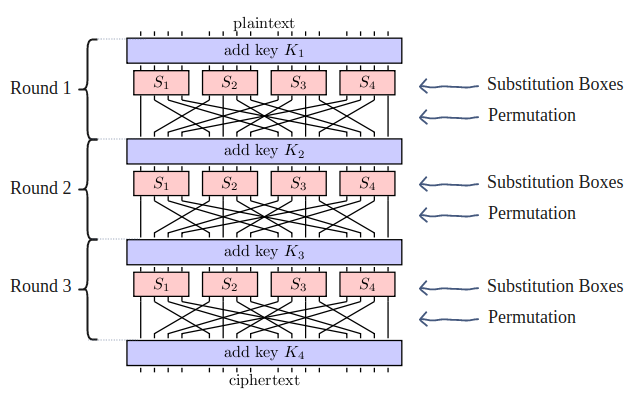
\includegraphics[width=0.5\textwidth]{images/spn.png}
  \caption{SPN structure.}
  \label{fig:spn}
\end{figure}

SPN structures consists of boxes called S-boxes that perform substitution operations and P-boxes that perform permutation operations. The S-boxes and P-boxes transform (sub-)blocks of input bits into output bits. Some common operations include simple and efficient XOR and bitwise rotation. \cite{mustafeez}

In the case of ASCON, the round transformation $p$ is based on an SPN structure. It consists of three main components: the constant addition  layer $p_C$, the substitution layer $p_S$, and the linear diffusion layer $p_L$. \cite{DBLP:journals/joc/DobraunigEMS21, ascon_specification} \par

\[p=p_C \circ p_S \circ p_L\]

In order to prepare the 320-bit state for the round transformations, the state is first divided into five 64-bit words. The round transformation $p$ is then applied to the state. \cite{DBLP:journals/joc/DobraunigEMS21} \par 

\begin{figure}[htbp]
  \centering
  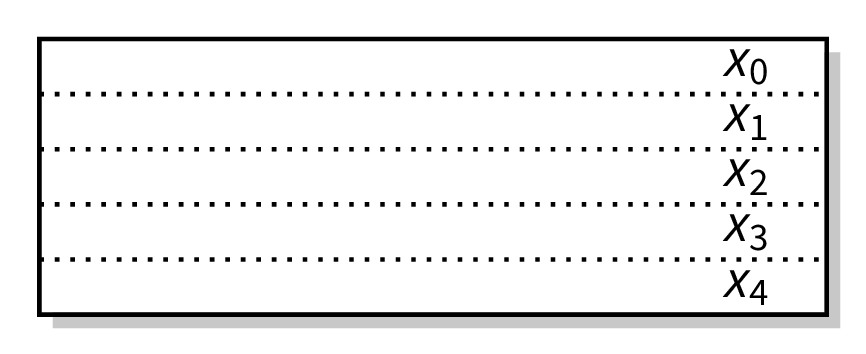
\includegraphics[width=0.5\textwidth]{images/state.png}
  \caption{The state divided into 5 64-bit words.}
  \label{fig:state}
\end{figure}

In each round of the permutation $p$ of ASCON, the following operations are performed:

\subsubsection{Constant addition layer $p_C$}
In $p_C$, a round specific 1-byte constant is XORed to $x_2$. \cite{ascon_specification, analysis_of_ascon}
  
\begin{figure}[htbp]
  \centering
  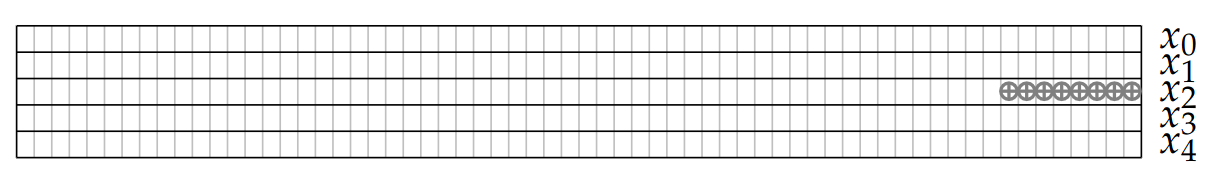
\includegraphics[width=0.8\textwidth]{images/constant.png}
  \caption{The constant addition layer $p_C$.}
  \label{fig:constant}
\end{figure}

\subsubsection{Substition layer $p_C$}
In $p_S$, a 5-bit S-box is applied to each byte of the state. It is the application of a 5-bit S-box 64 times in parallel vertically. \cite{ascon_specification, analysis_of_ascon}

\begin{figure}[htbp]
  \centering
  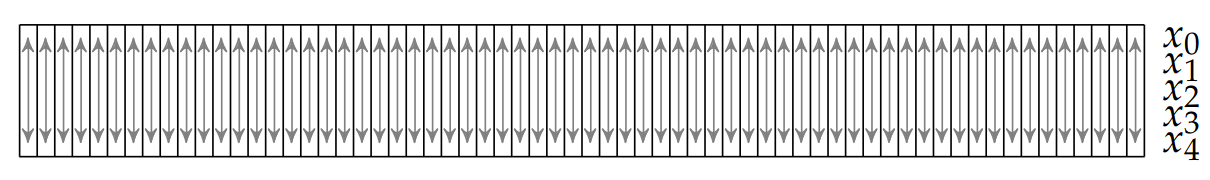
\includegraphics[width=0.8\textwidth]{images/substitution.png}
  \caption{The substitution layer $p_S$.}
  \label{fig:substition}
\end{figure}

\subsubsection{Diffusion layer $p_C$}
in $p_L$, a linear diffusion matrix is applied to the state which only consists of XOR and right rotation of the 64-bit words $x_0, x_1, x_2, x_3, x_4$. \cite{ascon_specification, analysis_of_ascon}

\begin{figure}[htbp]
  \centering
  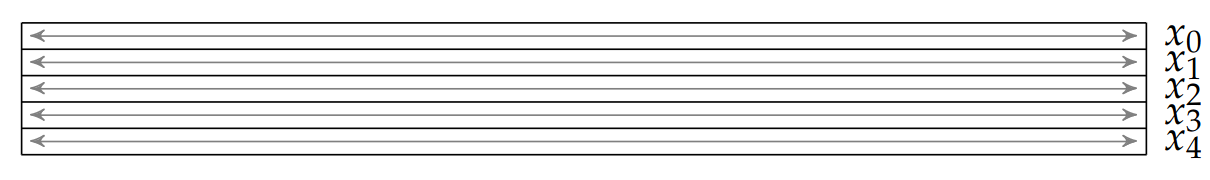
\includegraphics[width=0.8\textwidth]{images/diffusion.png}
  \caption{The diffusion layer $p_L$.}
  \label{fig:diffusion}
\end{figure}

The linear layer can be described as follows:


$\sum_0 (x_0) = x_0 \oplus (x_0 \ggg 19) \oplus (x_0 \ggg 28)$

$\sum_1 (x_1) = x_1 \oplus (x_1 \ggg 61) \oplus (x_1 \ggg 39)$

$\sum_2 (x_2) = x_2 \oplus (x_2 \ggg 1) \oplus (x_2 \ggg 6)$

$\sum_3 (x_3) = x_3 \oplus (x_3 \ggg 10) \oplus (x_3 \ggg 17)$

$\sum_4 (x_4) = x_4 \oplus (x_4 \ggg 7) \oplus (x_4 \ggg 41)$ 

\cite{ascon_specification,analysis_of_ascon}


\subsection{Design of the permutation}

There are several design criteria that need to be considered when designing a permutation for cryptographic purposes. In ASCON security was prioritised but also the performance was taken into account. \par

For the constant addition layer $p_C$, the round constants are chosen to prevent certain types of attacks and are added to the state in a simple, predictable manner for ease of computation. They are positioned strategically to facilitate efficient pipelining with other operations. \par

The S-box used in the substitution layer $p_S$ is carefully designed to meet various criteria, including invertibility, resistance against differential and linear cryptanalysis, and efficient implementation in hardware and software. \par

The linear diffusion layer mixes the bits within each word of the state. It is designed to resist linear and differential cryptanalysis while providing good diffusion. The rotation constants are chosen similar to those used in SHA-2 functions to balance performance and security. \par

\cite{DBLP:journals/joc/DobraunigEMS21}



\section{Conclusion}
In this paper, we have explored the critical aspects of lightweight cryptography, focusing on the unique requirements and challenges of securing resource-constrained environments. Through a detailed analysis of key cryptographic primitives—authenticated encryption, hashing, and permutations—we have highlighted the balance that must be achieved between security and efficiency.
\newline
The advancements in lightweight cryptography have shown significant promise, yet the field continues to face evolving threats and the need for robust, standardized solutions. The integration of new technologies, such as quantum computing, poses additional challenges that future research must address to ensure the continued security of lightweight cryptographic algorithms.
\newline
Our study underscores the importance of innovation and collaboration within the cryptographic community. By advancing lightweight cryptographic techniques, we can enhance the security of the growing ecosystem of connected devices, ensuring data integrity and confidentiality in an increasingly interconnected world.


\newpage
\printbibliography

\end{document}